%=====================================================================
\section{The data: cities, cars and requests}
\label{sec:data}

\subsection{Where the data comes from}

The instances are built from the \textbf{Solomon benchmark} (1987), the most used test set for vehicle routing with time windows. It has 56 files of 100 customers on a 100 $\times$ 100 grid, in six \emph{classes}:
\begin{itemize}
  \item \textbf{C} (clustered): customers in tight groups, like neighbourhoods;
  \item \textbf{R} (random): customers spread evenly over the city;
  \item \textbf{RC}: half clustered, half random.
\end{itemize}
Classes ending in \textbf{1} (C1, R1, RC1) have a \emph{short} planning period; classes ending in \textbf{2} have a \emph{long} one. The project turned each customer into a charging request (the \emph{EV-Solomon} dataset):
\begin{itemize}
  \item the Solomon \emph{ready time} becomes the request time $r_i$, and the depot's closing time becomes $T$ (unchanged);
  \item the Solomon \emph{demand} (1--50) becomes the energy need $E_i$ between 10 and 40 kWh;
  \item each car gets a remaining range of 5--40 km; 15\,\% of the cars are given less range than the distance to their nearest station (stranded);
  \item 12 stations are placed at the centres of the customer groups ($k$-means), 2 guns each; 5 vans at the depot.
\end{itemize}
Inside one class all files share the same positions, energies and ranges; only the request times differ. An \textbf{instance} is a file and its first $n$ cars, with $n=10,20,\dots,100$: 56 $\times$ 10 = \textbf{560 instances}, the same 560 for every method and every experiment.

\begin{table}[H]
\centering
\caption{The six Solomon classes as used here (one row per class; the EV attributes are those of the 100 cars of the class).}
\footnotesize
\begin{adjustbox}{max width=\linewidth}
\begin{tabular}{@{}lrrrrrrrrrr@{}}
\toprule
class & files & $T$ (min) & \shortstack{requests\\at 0 (\%)} & \shortstack{median\\$r/T$ (\%)} & \shortstack{mean $E$\\(kWh)} & \shortstack{stranded\\(\%)} & \shortstack{km to\\nearest FCS} & \shortstack{commercial\\(\%)} & \shortstack{mean $\theta$\\pers.} & \shortstack{mean $\theta$\\comm.} \\
\midrule
C1 & 9 & 1236 & 17 & 22 & 20.5 & 15 & 1.1 & 73 & 0.70 & 0.37 \\
C2 & 8 & 3390 & 19 & 29 & 20.5 & 15 & 1.6 & 69 & 0.72 & 0.39 \\
R1 & 12 & 230 & 25 & 23 & 18.3 & 15 & 1.9 & 70 & 0.64 & 0.37 \\
R2 & 11 & 1000 & 27 & 18 & 18.3 & 15 & 1.9 & 72 & 0.69 & 0.36 \\
RC1 & 8 & 240 & 19 & 25 & 19.9 & 15 & 1.8 & 66 & 0.73 & 0.35 \\
RC2 & 8 & 960 & 19 & 23 & 19.9 & 15 & 1.8 & 73 & 0.68 & 0.35 \\
\bottomrule
\end{tabular}
\end{adjustbox}

\end{table}

\begin{figure}[H]
\centering
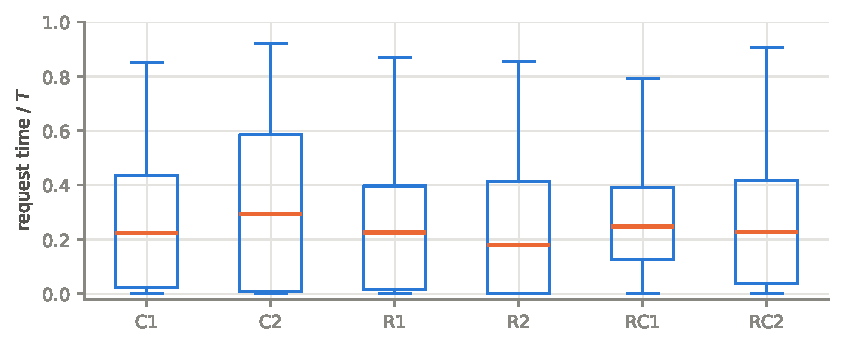
\includegraphics[width=0.85\textwidth]{figures/data_requests.pdf}
\caption{When requests arrive, as a share of the planning period $T$ (all cars of all files of each class). The box holds the middle half of the requests, the orange line is the median. About a fifth to a quarter of the requests arrive at minute 0.}
\label{fig:requests}
\end{figure}

What the table and the figure say, in words:
\begin{itemize}
  \item \textbf{The planning periods differ enormously}: R1 and RC1 have only 230--240 minutes, C2 has 3\,390. A charging session takes 27--109 minutes at a station, so in R1 and RC1 the chargers are very busy, while in C2 there is plenty of time.
  \item \textbf{Requests are spread over the whole period}, with a peak at the start (17--27\,\% at minute 0).
  \item \textbf{Every class has 15\,\% stranded cars}, which only a van can serve. With 5 vans of 6 seats there are 30 van seats; at $n=100$ about 15 of them are needed just for the stranded cars.
  \item \textbf{Stations are close}: the average car is 1--2 km from its nearest station.
\end{itemize}

\inshort{560 instances from the Solomon benchmark: six city types, short or long planning periods, 10 to 100 cars, 24 guns and 5 vans, and 15\,\% of cars that only a van can reach.}

%=====================================================================
\section{The two customer attributes: segment and income}
\label{sec:calib}

Each car carries two numbers that are written once into the dataset (\code{data/solomon\_data.csv}, columns \code{segment} and \code{theta}). The same car number has the same segment and income in every file of a class.

\subsection{Segment: 70\,\% commercial}

The model's customers are \emph{charging requests at public chargers}, not registered cars. Among electric four-wheelers registered in India in 2024 only about 10\,\% are cabs. But a cab drives about 5 times as far per day as a private car, and charges far more in public (about half of its energy, against about 10\,\% for private cars, most of whom charge at home). So a cab produces about 25 times as many public charging requests as a private car, and the share of commercial cars among requests is
\[
\pi_C=\frac{0.10\times25}{0.10\times25+0.90}=0.735,
\]
rounded down to \textbf{0.70}. In the dataset \fcomShareData\,\% of the cars are commercial.

\subsection{Income: rich private owners, lower-middle-income drivers}

\begin{itemize}
  \item \textbf{Personal cars}: about 14\,\% of urban households own a car, about 30\,\% in the richest fifth. If ownership rises with income as a power curve, the owners' income positions follow a Beta(2.5, 1) distribution (mean 0.71). Electric cars are dearer than average cars, so their owners are probably even richer; this is the least extreme choice the data allow.
  \item \textbf{Commercial cars}: surveys of app-based cab drivers report median net earnings of about Rs 15\,000 a month. That puts a driver's household around the 25th--50th income percentile: Beta(3, 5), mean 0.375. This is the least supported number and the first to replace when better data exist.
\end{itemize}

\begin{figure}[H]
\centering
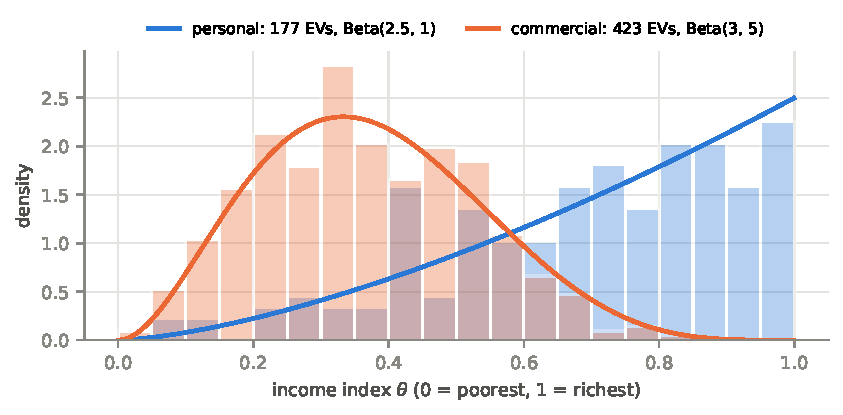
\includegraphics[width=0.85\textwidth]{figures/data_theta.pdf}
\caption{Income index of the cars in the dataset (bars: the 100 cars of each of the six classes; lines: the calibrated Beta distributions). Mean $\theta$: personal \fthetaPersData, commercial \fthetaComData. The customer population is two-humped: rich private owners and lower-middle-income drivers.}
\label{fig:theta}
\end{figure}

\inshort{Seven out of ten requests come from taxis and fleet cars, whose drivers are mostly lower-middle income; the remaining three come from mostly rich private owners.}

%=====================================================================
\section{The customer parameters}

Each sensitivity is a straight line in $\theta$, from its value at $\theta=0$ to its value at $\theta=1$, with separate end points for each segment (\code{common/f4\_params.json}).

\begin{table}[H]
\centering
\caption{End points of the customer lines. Every customer's own value is read off the line of its segment at its $\theta$.}
\small
\begin{adjustbox}{max width=\linewidth}
\begin{tabular}{@{}lrrrr@{}}
\toprule
quantity & personal $\theta=0$ & personal $\theta=1$ & commercial $\theta=0$ & commercial $\theta=1$ \\
\midrule
money sensitivity $\mu$ & 1.5 & 0.5 & 1.5 & 0.5 \\
drive to FCS $c^{D}$ (Rs/min) & 1.5 & 15 & 1.5 & 6 \\
queue at FCS $c^{Q}$ (Rs/min) & 2.5 & 25 & 2 & 7.5 \\
charge at FCS $c^{C}$ (Rs/min) & 1 & 10 & 1.5 & 6 \\
wait for / charged by van $c^{V}$ (Rs/min) & 0.5 & 5 & 1.5 & 6 \\
longest queue $W$ (min) & 60 & 15 & 40 & 15 \\
\bottomrule
\end{tabular}
\end{adjustbox}

\end{table}

\begin{figure}[H]
\centering
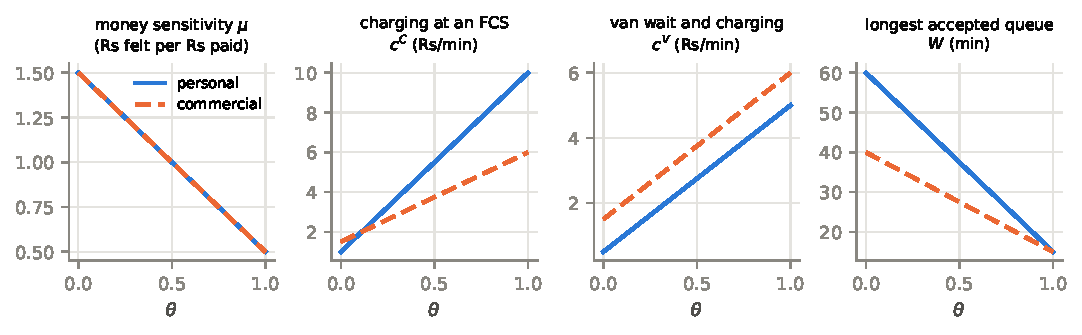
\includegraphics[width=\textwidth]{figures/data_lines.pdf}
\caption{The customer lines (blue: personal, orange dashed: commercial). Money sensitivity is the same for both segments. A personal driver's station minute gets very dear with income, while a van minute stays cheaper (driver-free). A commercial driver pays the same downtime rate for both (and it is higher than the personal van-minute value at every income).}
\label{fig:lines}
\end{figure}

How to read the lines:
\begin{itemize}
  \item \textbf{Money sensitivity $\mu$} falls from 1.5 (poorest) to 0.5 (richest), the same in both segments: a poor customer feels a rupee three times as much as a rich one.
  \item \textbf{Personal values of time} rise steeply with income: a rich owner's station minute costs Rs 10, a van minute only Rs 5 (driver free).
  \item \textbf{Commercial values of time} are one downtime rate from Rs 1.5 to Rs 6 per minute, the same for drive, station charging and van; queueing Rs 2--7.5.
  \item \textbf{Queue tolerance $W$}: 60 minutes for the poorest private owner, 40 for the poorest driver, 15 for the richest of both.
  \item \textbf{Tariffs}: Rs \fpF/kWh at a station, Rs \fpM/kWh for a van (a premium of Rs 10/kWh for charging at the door).
\end{itemize}

\inshort{Except for the segment share and income distributions, these numbers are reasoned guesses. The experiments test how much the results depend on the most important of them.}

%=====================================================================
\section{The experiments and the data each one uses}
\label{sec:experiments}

Each experiment changes \textbf{one} input and solves the same 560 instances again with both methods. Nothing else changes: same cars, same positions, same request times, same segments and incomes. No data files are copied: the solver reads \code{data/} and applies the change in memory (for example \code{--set tariff\_Rs\_per\_kWh.p\_M=35}).

\begin{table}[H]
\centering
\caption{The 15 variants of the five experiments.}
\footnotesize
\begin{adjustbox}{max width=\linewidth}
\begin{tabular}{@{}l>{\raggedright\arraybackslash}p{4.3cm}>{\raggedright\arraybackslash}p{5.6cm}>{\raggedright\arraybackslash}p{3.6cm}@{}}
\toprule
exp. & variant id & what is changed & baseline value \\
\midrule
E5 & E5\_\allowbreak cC1\_\allowbreak personal\_\allowbreak 7.5 & personal $c^{C,1}$ = 7.5 ($-$25 \%) & personal $c^{C,1}$ = 10, commercial $\omega^1$ = 6 \\
 & E5\_\allowbreak cC1\_\allowbreak personal\_\allowbreak 12.5 & personal $c^{C,1}$ = 12.5 ($+$25 \%) &  \\
 & E5\_\allowbreak omega1\_\allowbreak commercial\_\allowbreak 4.5 & commercial downtime rate at $\theta=1$: 4.5 ($-$25 \%) &  \\
 & E5\_\allowbreak omega1\_\allowbreak commercial\_\allowbreak 7.5 & commercial downtime rate at $\theta=1$: 7.5 ($+$25 \%) &  \\
\midrule
E6 & E6\_\allowbreak mu0\_\allowbreak personal\_\allowbreak 1.125 & personal $\mu^0$ = 1.125 ($-$25 \%) & personal $\mu^0$ = 1.5, commercial $\mu^0$ = 1.5 \\
 & E6\_\allowbreak mu0\_\allowbreak personal\_\allowbreak 1.875 & personal $\mu^0$ = 1.875 ($+$25 \%) &  \\
 & E6\_\allowbreak mu0\_\allowbreak commercial\_\allowbreak 1.125 & commercial $\mu^0$ = 1.125 ($-$25 \%) &  \\
 & E6\_\allowbreak mu0\_\allowbreak commercial\_\allowbreak 1.875 & commercial $\mu^0$ = 1.875 ($+$25 \%) &  \\
\midrule
E1 & E1\_\allowbreak pM\_\allowbreak 15 & $p^M$ = 15 Rs/kWh (= $p^F$) & $p^M$ = 25 \\
 & E1\_\allowbreak pM\_\allowbreak 35 & $p^M$ = 35 Rs/kWh &  \\
\midrule
E2 & E2\_\allowbreak vans\_\allowbreak 3 & 3 vans & vans = 5, seats = 6 \\
 & E2\_\allowbreak vans\_\allowbreak 7 & 7 vans &  \\
 & E2\_\allowbreak seats\_\allowbreak 4 & 4 EVs per van &  \\
 & E2\_\allowbreak seats\_\allowbreak 8 & 8 EVs per van &  \\
\midrule
E8 & E8\_\allowbreak battery\_\allowbreak 200 & B = 200 kWh & battery = 150 \\
\bottomrule
\end{tabular}
\end{adjustbox}

\end{table}

\begin{description}[leftmargin=1em]
  \item[E5 Value of charging time.] The value of a personal owner's station minute at the top income ($c^{C,1}$, the most influential guess in formulation 3), and separately the commercial downtime rate at the top income ($\omega^1$; drive, station and van minutes all change with it, queueing too). $\pm25$\,\%. \emph{Question:} how much does each segment's use of vans depend on this guess? \emph{Theory:} the personal change should move the personal van share; the commercial change should move the cost but hardly the van share.
  \item[E6 Money sensitivity.] How strongly the poorest customer feels a rupee ($\mu^0$), separately for each segment, $\pm25$\,\%. \emph{Question:} the same for the coefficient with the largest effect on $Z$. \emph{Theory:} it changes the felt cost of every tariff and drive, so $Z$ moves directly; it matters most for the segment with many poor customers (commercial).
  \item[E1 Van tariff.] $p^M$ = 15 (equal to the station price: no premium) and 35 (double premium), baseline 25. \emph{Question:} who gets vans, and what does it cost the operator and the customers? \emph{Theory:} without a premium the money reason against vans disappears, so van use rises, mostly among personal owners.
  \item[E2 Van fleet and seats.] 3 or 7 vans (baseline 5); 4 or 8 cars per van (baseline 6), one change at a time. \emph{Question:} where does another van or seat pay off?
  \item[E8 Van battery.] 200 kWh instead of 150. \emph{Question:} is van recharging worth modelling? Decision rule set in advance: if $Z$ moves by less than 1\,\%, no.
\end{description}

\textbf{How a variant is compared with the baseline.} Only on \emph{paired instances} (valid in both). For each, the change of $Z$ in \%; then the mean. The van share is pooled over all free-choice cars of the paired instances. Instances that gain or lose a valid plan are counted separately (\emph{new} and \emph{lost}).

\inshort{Five experiments, 15 variants, each changing one number; everything else, including all the data, stays the same.}
